\documentclass{article}
    % General document formatting
    \usepackage[parfill]{parskip}
    \usepackage[utf8]{inputenc}
    \usepackage{fullpage}
    \usepackage{geometry}
    \usepackage{graphicx}
    % Related to math
    \usepackage{amsmath,amssymb,amsfonts,amsthm}

\begin{document}
\section*{Title}
@paper
\section*{Abstract}
@paper
\section*{Keywords}
Artificial Intelligence, Constraint Programming, Explanation

\section*{Suggested reviewer list}
\begin{figure}[h!]
    \centering
    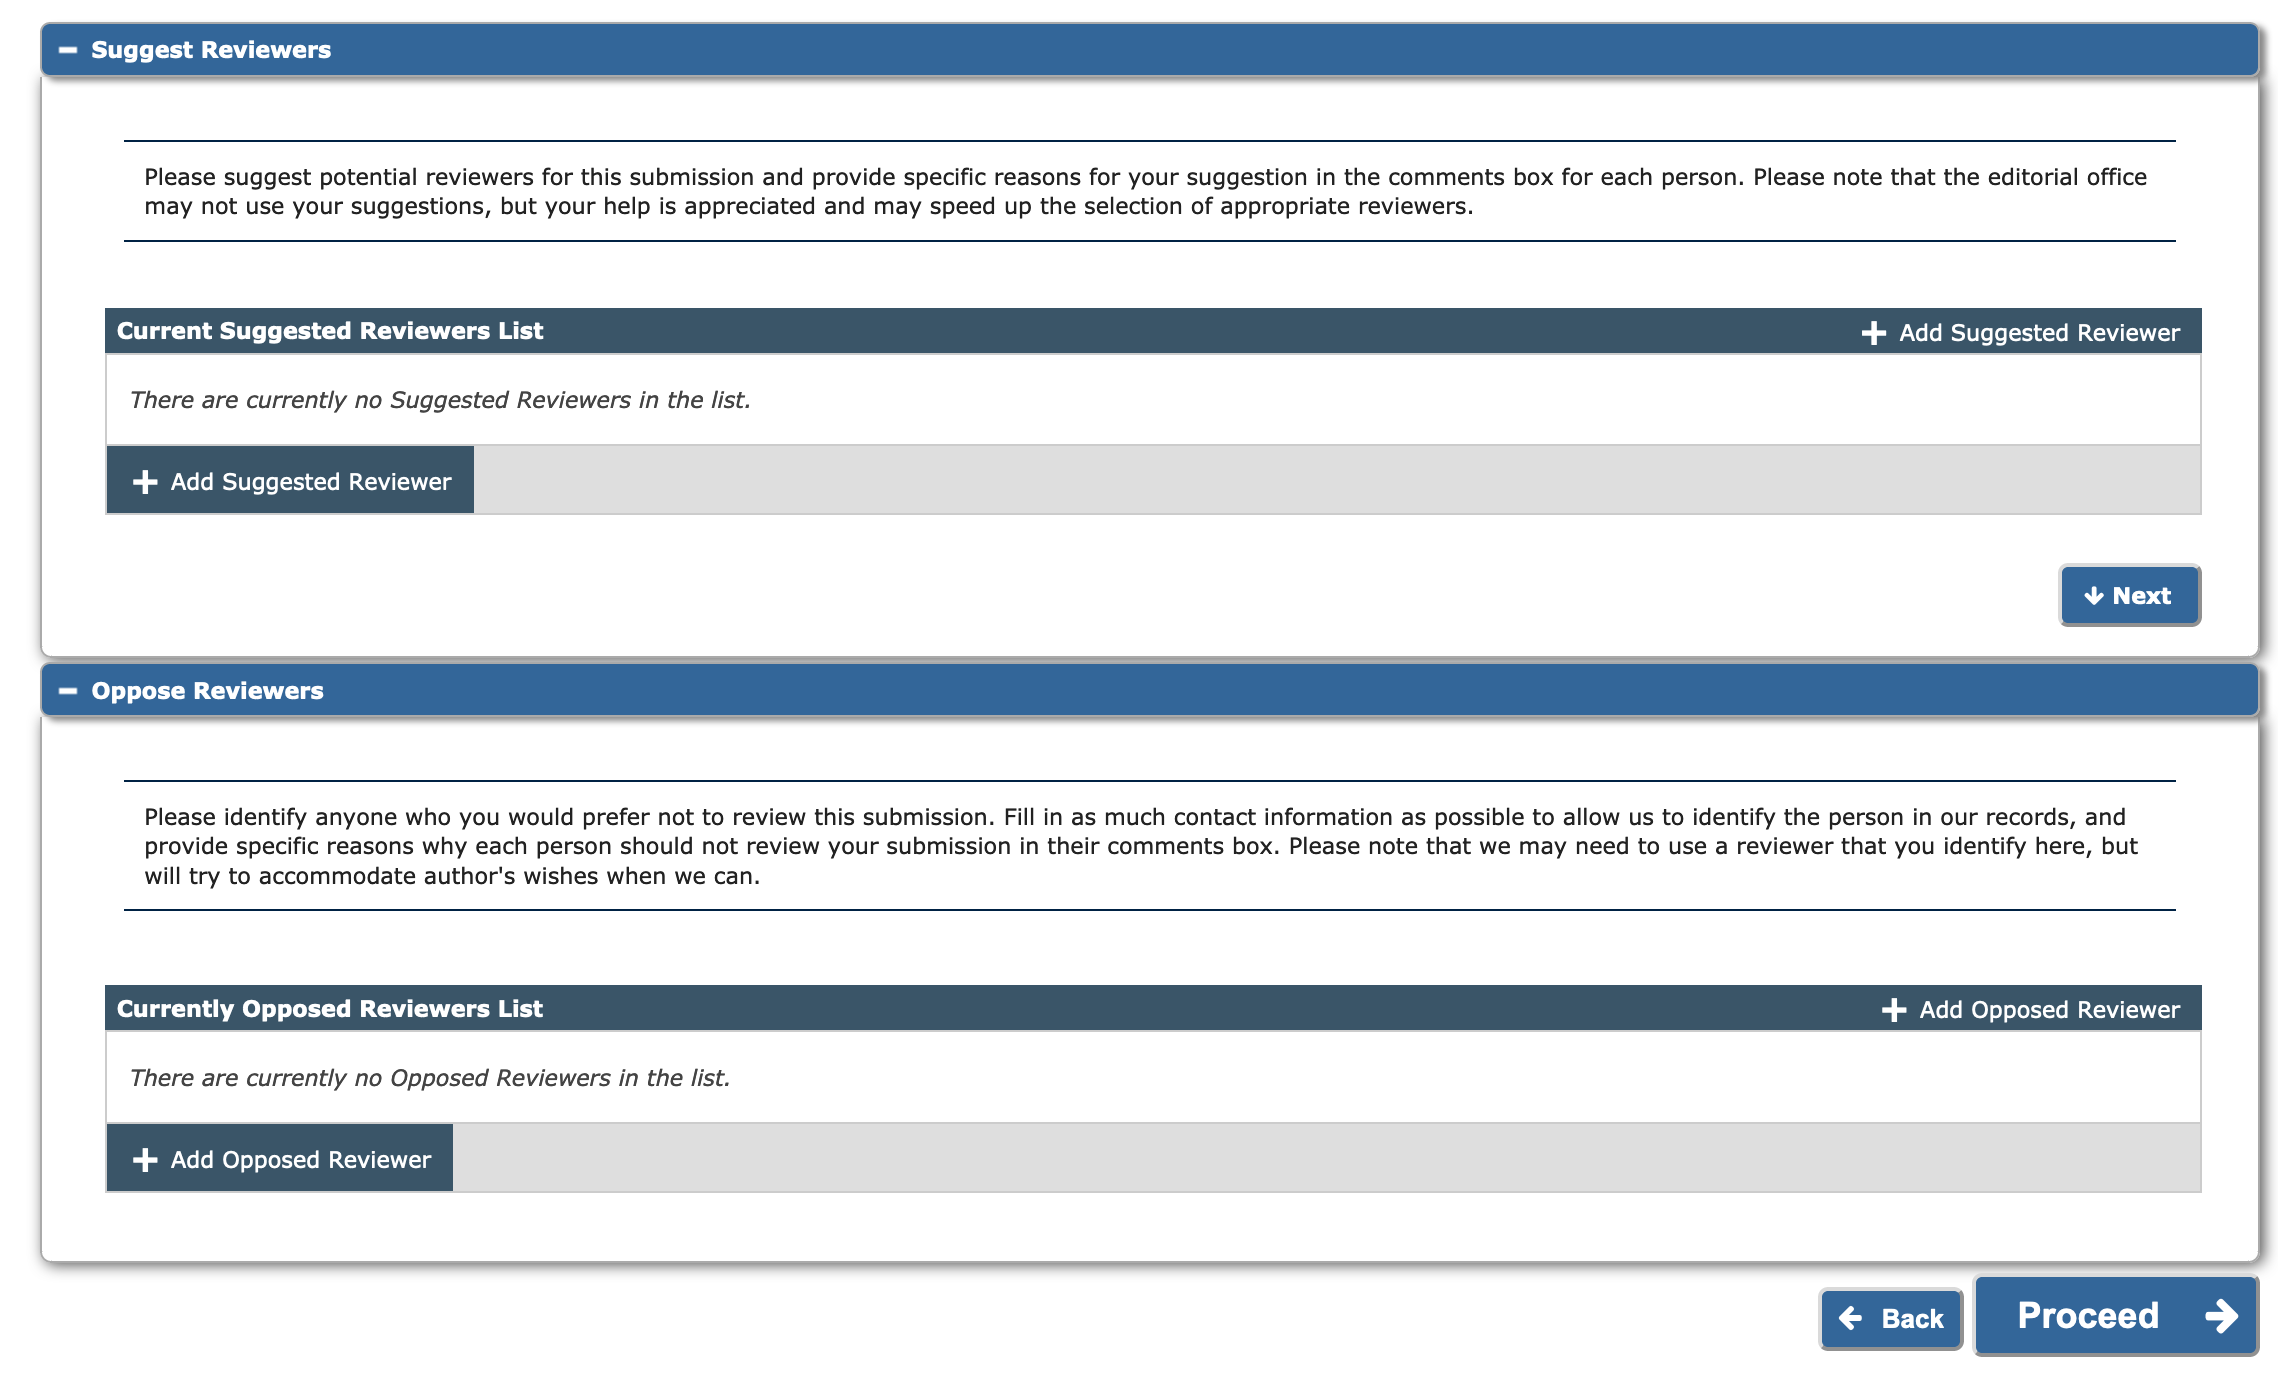
\includegraphics[width=\textwidth]{reviewers}
\end{figure}

Hmmm... I don't have anyone to oppose. 
Suggested: is a strategic decision: who would like and appreciate this work? 

\section*{Questions additional information}
\subsubsection*{If any part of this work has been submitted or published elsewhere, please state where it has been submitted and how it differs from the paper submitted here. (Please either confirm that that the work has not been submitted or published elsewhere, or give details)}

This paper is an extension of a couple of previous papers presented at workshops and conferences \cite{claesuser,DBLP:conf/bnaic/ClaesBCGG19,ecai/BogaertsGCG20}. The current paper extends the previous papers we more detailed examples, additional experiments, as well as a formal treatment of what we call \emph{nested explanation sequences} (an idea that first appeared in a demo we submitted to IJCAI-PRICAI 2020 but that is first formalized in the current paper).  




\subsubsection*{Do you agree not to submit the paper elsewhere during the review period? (We will not review papers without an affirmative answer.) (Please answer the question with a YES / NO)}

YES


\subsubsection*{What is, in one or two sentences, the original contribution of this work?}

We formalize the problem of step-wise explaining the propagation of a constraint solver through a sequence of small inference steps, and define an abstraction mechanism for this framework. 
We develop algorithms that generate such explanations and validate our approach on logic grid puzzles. 


\subsubsection*{Why should this contribution be considered important for the field of Artificial Intelligence? Please confirm where you explain this in the paper?}

This paper fits in the research line of ``Explainable AI'' and thus is a highly relevant fit for AIJ (especially the current special issue). This is explained in the introduction. 


\subsection*{What is the most closely related work by others, and how does this work differ? Please give 1-3 citations to such papers (not papers that of yours or your co-authors, of course), preferably from outlets such as the AI journal, the Journal of Artificial Research, IJCAI, AAAI, ECAI or some similar quality artificial intelligence venue. Your related work section should discuss the relationship in more detail.}

Explainable planning paper

QuickXplain? 

Freuder's work?




\subsubsection*{AIJ will publish only work that is relevant to AI. It must also be accessible to a wide audience, even if the contribution of the paper is a narrow technical one (i.e. other AI researchers, not necessarily in the same sub-field should be able to appreciate the results and understand the paper's contributions and its relevance to AI). Your paper will be sent back for revisions or rejected if this is not the case. Answer the following two questions:}

\begin{enumerate}
    \item Is your work relevant to AI, and where do you explain the relevance to AI in the paper? Yes. In the introduction. 
    \item Can you confirm that at least the abstract, introduction and conclusion can be appreciated by a general AI audience? Yes. 
\end{enumerate}


\subsubsection*{AIJ encourages authors to submit additional electronic material (data sets, programs, videos....) which would be published in Science Direct if the paper is accepted (though not in the print version). Please describe here any such material you would make available in this way.}

Nothing? 

\subsubsection*{Did the availability of the AI journal for free as detailed at http://aij.ijcai.org/free-access-to-the-ai-journal influence your decision to submit to the AI journal?}

No?

\section*{Comments ? }
\subsubsection*{ Please enter any additional comments you would like to send to the publication office. These comments will not appear directly in your submission. }

\section*{funding}


\begin{figure}[h!]
    \centering
    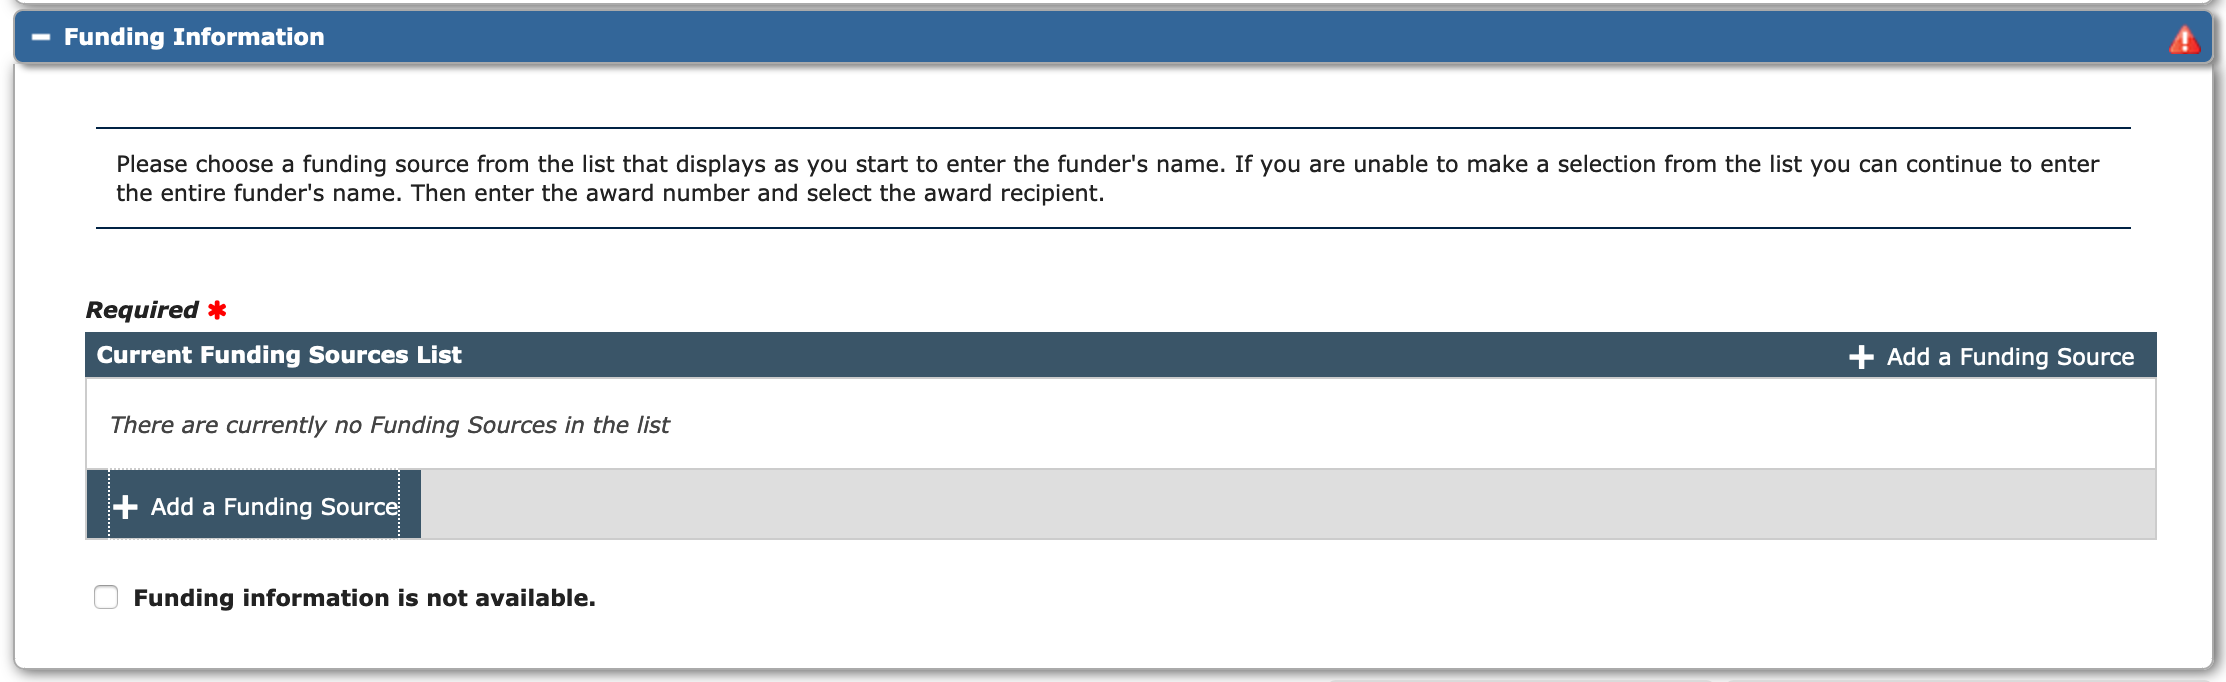
\includegraphics[width=\textwidth]{funding}
\end{figure}

Flemish gov (see paper)

\end{document}
